%!TEX root = ../master.tex
\chapter{Background Research}\label{ch:bgresearch}



\section{Types of Sources}\label{sec:typesofsources} 
The sources used in this chapter include scientific articles regarding the topic “Image to sound conversion”. The articles are published in the fields of physics, sound art and digital media. Other sources include recorded lectures of one of the articles authors.

\section{Previous work}\label{sec:previouswork}

\subsection{An Experimental System for Auditory Image Representation}\label{sec:experimentalsystem}

To interpret an image, humans are naturally born with visual sense. However, if the visual sense is missing for an individual, the visual image is not perceivable. This allows for a technical replacement which can provide the individual with a tool to substitute the missing sense or enhance other senses which are still functional. An experimental system for vision substitution was developed by Peter B. L. Meijer\cite{Meijer1992}. The system consists of a computer connected to a camera, which records real-time images and converts them into sound. 

The system used a method called time-multiplexed mapping, where the distribution of rows and columns in an image, the height (M) and width (N) respectively, where the pixels are stored in a matrix. The time spent scanning the image(R) is used to define when the current image ends and the next image begins. An example of this method is seen in Figure \ref{fig:image_to_sound}. 

\begin{figure}[!h] 
\centering
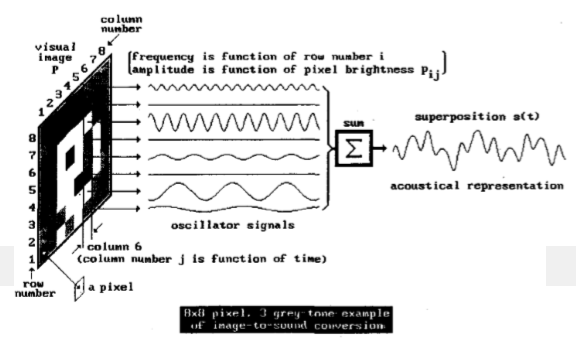
\includegraphics[width=1\textwidth]{image_to_sound}
\caption{\label{fig:image_to_sound} Principles of the image-to-sound mapping \cite{Meijer1992}}
\end{figure}
\cite{Meijer1992}

\todo{add reference[comment: to what?]}
  
The images have a resolution of 64 * 64 pixels with 16 gray-tones per pixels.  

The experiment showed promising functionality to convert images to sound but lacks a field study test on people with blindness. Moreover, the advantages and disadvantages of this system is yet to be proved. This questions the reliability of the system since there is no recordings of testing data presented in the article of the experiment. However theory supports the system's functionality. The operations used in the system can also be applied in other settings than an aid for blind individuals, as these operations are mathematical expressions. They are therefore not limited to the use intended by Meijer.

\subsection{The Sound of Photographic Image}\label{sec:soundarticle}

A use of images for conversion into sound was performed and described in a paper by Atau Tanaka, who is the chair of digital media and director of culture lab at Newcastle University \cite{Tanaka2012}.

The paper describes two processing methods that both converts images into sound.

The first method utilises two image series. The method used to create the sound from the image uses a temporary mapping and additive synthesis on raw grayscale images, by scanning every pixel. A bright pixel produces high notes and a dark pixel produces a low note \cite{Tanaka2012}.

The second method was used for an interactive art installation. The interactive art consisted of a wooden structure with panels covered in rice paper to display Tanaka's pre-processed images from one of the image series. The images were processed through re-synthesis processes, where the frequency bands where quantisized to whole tones and pentatonic were mapped in which the key notes are played one at a time. The images were projected with negative pixel values creating a inverted image of the original and each row displayed different frequency ranging from low to high frequencies. An example of this result can be seen in Figure \ref{fig:tanakaresynthesis}.  

\begin{figure}[!h]
\centering
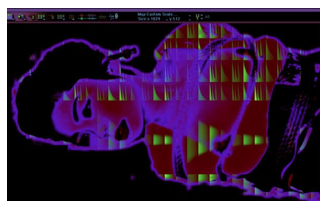
\includegraphics[width=1\textwidth]{tanakaresynthesis}
\caption{\label{fig:tanakaresynthesis}\cite{Tanaka2012}}
\end{figure}
\cite{Tanaka2012}

To capture human interaction, an infrared camera on top of the installation used viewers silhouettes as a layer on the negative image which was used to reveal the original black and white image for the viewer, as seen in Figure \ref{fig:tanakainterfacepreview}.

\begin{figure}[!h]
\centering
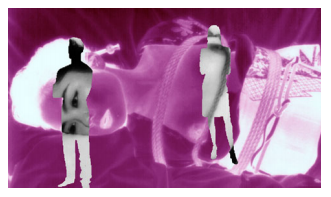
\includegraphics[width=1\textwidth]{tanakainterfacepreview}
\caption{\label{fig:tanakainterfacepreview}\cite{Tanaka2012}}
\end{figure}

This interaction also affected the produced sound which were based on the brightness of the processed image and thus produced new sounds. 

This visualisation of sound through images shows dynamic functionality of a interactive system, which utilises human interaction to alter a preprocessed image. However, since there was no evaluation of this exhibit, it is difficult to know of the practical application of these methods. This is due to it being used in an artistic way, instead of a practical one.   

\section{Methods used to evaluate}\label{sub:methodsusedtoevaluate}

\subsection{Volterra series}\label{sub:Volt}

\todo{look through this with Victor}

The Volterra series is an extension of the linear systems theory, which uses linear operators in signal processing \todo{add reference to linear systems theory}. The Volterra series can calculate the high-frequency-low-distortion terms for any weakly non-linear time-invariant (NLTI) system with memory effect.  The input and output signals allow the calculation of the linear impulse response defined as h_1(n) by cross-correlation and kernels (impulse responses). The linear impulse response has many variations defined as h_1(n) in a one-dimensional or a two-dimensional h_2(n_1, n_2) and h_N(n_1 …., n_N) is an N-dimensional kernel. The N-kernels can be used for an N-order Volterra system model. 

\todo{Add functionen i bogen}

However, the Volterra series has a hard time with strongly non-linear problems where the sum will go in different directions and therefore difficult to determinate. 


\section{State of the art}\label{sec:stateart}
In this project, software that allows images to be converted into sounds are to be considered as the state of the art, as they are closely related to the topic of the project.

\subsection{SonicPhoto}\label{sub:sonic}
!Anna rewritten!
SonicPhoto \cite{White2013} is a commercial piece of software developed for windows that allows a user to input an image and converts it into unique sounds. The software interprets the image as a spectrogram, having pitch on the y-axis and time on the x-axis. The intensity of the pixels is interpreted as the amplitude of the sound. 

The software allows for customisation, such as being able to change the note harmonics, which cord nodes are played, the base of the pitch, the lowest and highest frequencies. It is also possible to edit the image; changing the alpha, rotation, flipping it on the x or y-axis, and inverting the colours. 

\todo{more general information about the program. Which points to we want to make, by writing about this program?}

\subsection{Metasynth}\label{sub:metasynth}
MetaSynth, a software for OSX, is also an image-to-sound conversion software. It resembles SonicPhoto by being able to import an image and edit it by for example flipping, rotating, adjusting gamma, blurring. However, MetaSynth has additional functionality for editing the output sound, as the user can add effects like  convolution, grain, delay, reverb, and chorus. The image is interpreted as a spectrogram by the software.
There is also the possibility to draw freely on the image, while still having all the previously mentioned customisation for both image and sound. In this software, the color of the image determines the stereo placement. Green color for the right stereo, red for the left stereo and yellow in the center. Intensity determines the amplitude. 
Compared to SonicPhoto, MetaSynts emphasises on making musicm in addition to just making sounds. This is because the program allows for adding or putting the audio that the user has created into a sequence to create longer soundtracks.